Идентификация авторов исходного кода производилась на основании различных признаков, которые каким-либо 
образом могут идентифицировать так называемый стиль написания программ, присущий конкретному автору. 
Помимо деанонимизации автора, стиль написания кода может дать представление об уровне его квалификации, 
образовании, личных и профессиональных предпочтениях, а также некоторых других особенностях, которые могут 
представлять интерес в различного рода исследованиях. 

Перечисленные в данном разделе признаки являются характерными для языков C и С++, однако могут быть 
использованы для исследования C-подобных языков, например, D, Java, Objective C, C\#, PHP, perl и другие.

\subsection{Лексические признаки}

Главная особенность данной группы признаков состоит в том, что они могут быть вычислены при 
непосредственном анализе исходного кода программы в виде текстового файла. 
При этом код программы может быть некомпилируемым, неполным, содержащим
синтаксические или программные ошибки.

Лексические признаки включают в себя:

\begin{itemize}
 \item Стиль комментирования --- данная подгруппа определяет преобладающий в тексте вид комментариев 
 (однострочные или многострочные), а также общее их количество.
 \item Стиль расстановки фигурных скобок --- к наиболее известным относят <<K\&R>>, <<Whitesmith>>, 
<<One True Bracing Style>>, стиль Алмена и другие.~\cite{bracing_styles} 
 
 \item Стиль 
\end{itemize}



В таблице~\ref{tab:1} приведено описание использованных при классификации авторов 
признаков.

\begin{table}[h!]
\caption{ Лексические признаки }
\label{tab:1}
\begin{center}
\begin{tabularx}{\linewidth}{|X|X|X|}
\hline
\multicolumn{3}{|c|}{Лексические признаки} \\
\hline
\multicolumn{1}{|c|}{Признак} & \multicolumn{1}{|c|}{Обозначение} & \multicolumn{1}{|c|}{Определение} \\
\hline
Число комментариев & ln\_comments & Натуральный логарифм отношения числа комментариев к длине файла в символах \\
\hline
Число макросов & ln\_macros & Натуральный логарифм отношения числа макросов к длине файла в символах \\
\hline
Число пробелов & ln\_spaces & Натуральный логарифм отношения числа пробелов к длине файла в символах \\
\hline
Число символов табуляции & ln\_tabs & Натуральный логарифм отношения числа символов табуляции к длине файла в символах \\
\hline
Число переводов строки & ln\_newlines & Натуральный логарифм отношения числа переводов строки к длине файла в символах \\
\hline
Коэффициент пробельных символов & whitespace\_ratio & Натуральный логарифм отношения суммы всех пробельных символов (пробелов, символов табуляции, переводов строки) к длине файла в символах \\
\hline
Число строк кода & lines\_of\_code & Число строк кода, не включающее пустые строки\\
\hline
\end{tabularx}
\end{center}
\end{table}



\subsection{Ключевые слова С++}\label{keycpp}

Ключевые слова С++ представляют собой список зарезервированных последовательностей символов, используемых языком, недоступных для переопределения.

Для ключевых слов языка С++ вычислялась статистическая мера TF (term frequency), отображающая число вхождения некоторого слова к общему количеству слов в документе. Словарь из 84 ключевых слов С++ (стандарт 11) был взят на сайте с официальной документацией~\cite{cppkeywords} и представлен в таблице~\ref{tab:3}.

\begin{table}[ht]
\caption{ Ключевые слова языка С++ (стандарт 11) }
\label{tab:3}
\begin{center}
\begin{tabularx}{\linewidth}{|X|X|X|X|X|X|}
\hline
\multicolumn{6}{|c|}{Ключевые слова языка С++} \\
\hline
alignas & char32\_t & enum & namespace & return & try\\
alignof & class & explicit & new & short & typedef\\
and & compl & export & noexcept & signed & typeid\\
and\_eq & const & extern & not & sizeof & typename\\
asm & constexpr & false & not\_eq & static & union\\
auto & const\_cast & float & nullptr & static\_assert & unsigned\\
bitand & continue & for & operator & static\_cast & using\\
bitor & decltype & friend & or & struct & virtual\\
bool & default & goto & or\_eq & switch & void\\
break & delete & if & private & template & volatile\\
case & do & inline & protected & this & wchar\_t\\
catch & double & int & public & thread\_local & while\\
char & dynamic\_cast & long & register & throw & xor\\
char16\_t & else & mutable & reinterpret\_cast & true & xor\_eq\\
\hline
\end{tabularx}
\end{center}
\end{table}

% \newpage 
\subsection{Статистическая значимость признаков}
В ходе вычислительных экспериментов выяснилось, что только четверть из всего набора признаков (см. раздел~\ref{features}) встречалась в данном наборе тестовых данных (см. раздел~\ref{test_data}). Остальные признаки отсутствовали, т.е. их значения для данной выборки были нулевыми. Поскольку алгоритм классификации Random Forest базируется на методе случайных подпространств (см. раздел~\ref{random_forest}), признаки, по которым строятся деревья решений для дальнейшей классификации, выбираются случайным образом. Как следствие, при выборе признаков из всего изначального их набора приводит к тому, что построение деревьев решений производится в преимущественной доли случаев на нулевых значениях признаков и приводит к существенному снижению точности классификации. Данная проблема была решена обрезанием статистически незначимых признаков на каждой новой итерации классификации.  

График, отображающий статистически значимые признаки для используемого набора данных можно увидеть на рисунке~\ref{important:important}.

\begin{figure}[h!]
\center{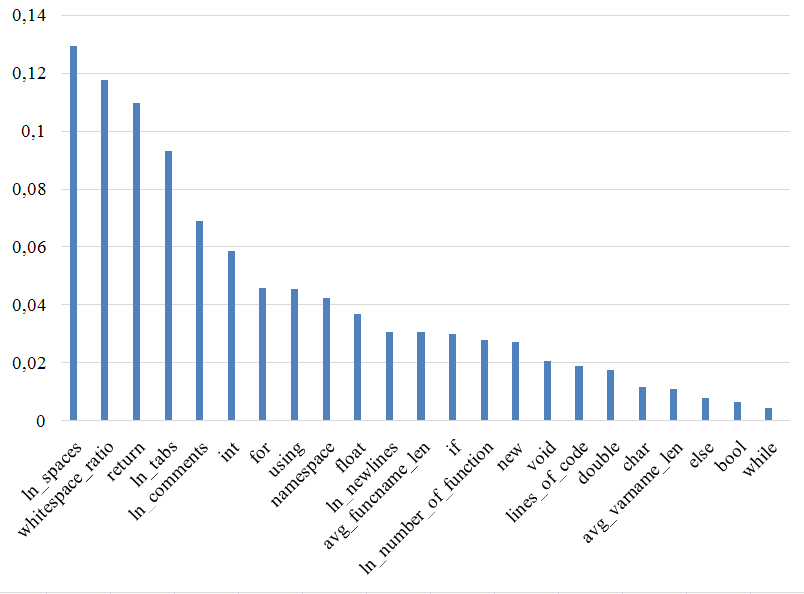
\includegraphics[width=0.9\linewidth]{important}}
\caption{ Статистически значимые признаки}
\label{important:important}
\end{figure} 
